\section{Physische Testumgebung}

Die physische Testumgebung für die Implementierung und Evaluierung der vorliegenden Arbeit besteht aus einer realen ChargeIQ-Wallbox. Die Detection-Module sind in diesem Szenario abweichend von der in Kapitel "Systemüberblick und verteilte Kommunikation"~\ref{sec:systemueberblick_und_verteilte_Kommunikation} beschriebenen Zielarchitektur nicht auf einem Raspberry Pi Zero 2 W, sondern zu Testzwecken auf einem leistungsfähigeren Raspberry Pi 4 B oder BananaPi M5 installiert. Diese sind über eine kabelgebundene Ethernet-Verbindung in das private IPFS-Netzwerk eingebunden, um eine stabile und performante Kommunikation zu gewährleisten. Die Wallbox selbst ist ebenfalls über eine drahtlose Verbindung in dasselbe private IPFS-Netzwerk integriert.

Darüber hinaus besteht eine serielle \textit{I2C}-Verbindung (\textit{Inter-Integrated Circuit}) zwischen der ChargeIQ-Wallbox und einem Einplatinencomputer in diesem fall der Raspberry Pi 4 B, welcher stellvertretend für die spätere Detection Unit auf Basis des Raspberry Pi Zero 2 W fungiert. Diese Verbindung ermöglicht die Erfassung von Echtzeitdaten des integrierten Wattmeters, welcher die sensor daten für eine im Kapitel "Detection Units der Ladeinfrastruktur"~\ref{sec:detection_units_der_ladeinfrastruktur} beschriebene Detektionseinheit bereitstellt.

Zusätzliche Sensordaten werden dem Raspberry Pi 4 B über die in der Testumgebung eingerichtete drahtlose WLAN-Verbindung übermittelt, in welche sowohl die als Detection Unit eingesetzte Einplatinencomputer als auch die Wallboxen eingebunden sind.

\begin{figure}[H]
    \centering
    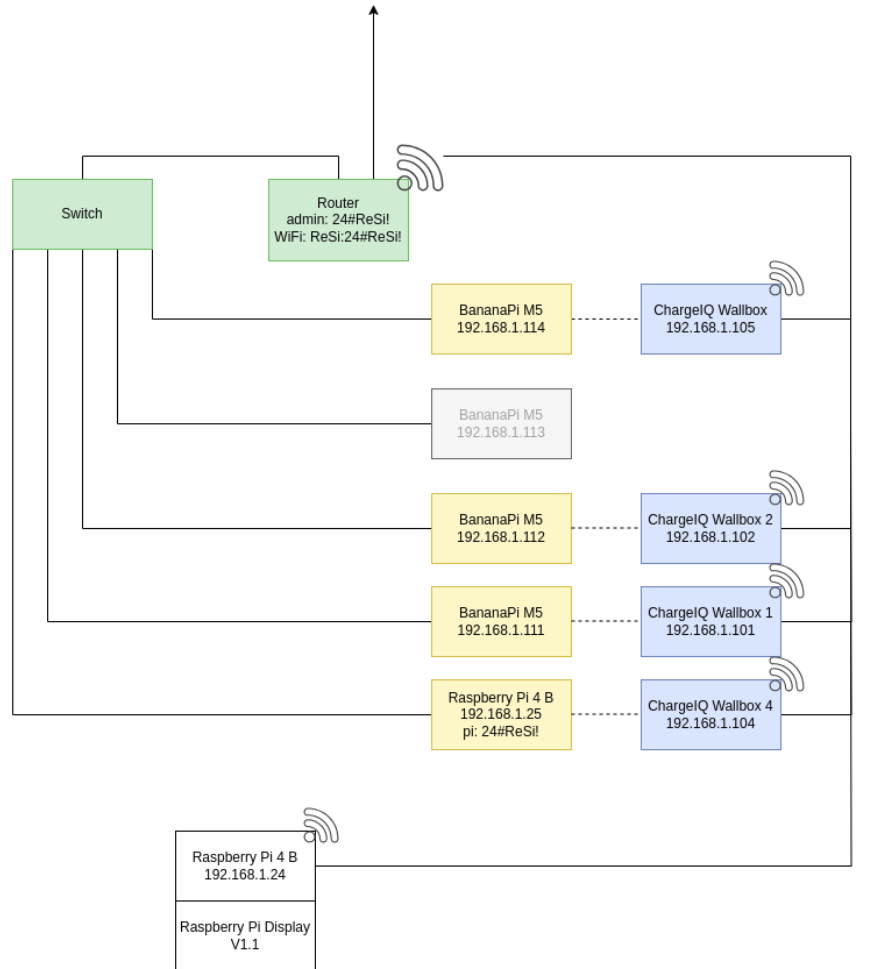
\includegraphics[width=0.75\textwidth]{./figures/SystemDiagramv2.drawio.png}
    \caption{Schematische Darstellung der physischen Testumgebung.}
    \label{fig:SystemDiagramv2}
\end{figure}